\documentclass[12pt,a4paper]{article}

% ── Packages ─────────────────────────────────────────────────────────────────
\usepackage[T1]{fontenc}
\usepackage[utf8]{inputenc}
\usepackage{lmodern}
\usepackage[margin=2.5cm]{geometry}
\usepackage{graphicx}
\usepackage{xcolor}
\usepackage{hyperref}
\usepackage{listings}
\usepackage{booktabs}
\usepackage{tabularx}
\usepackage{longtable}
\usepackage{caption}
\usepackage{subcaption}
\usepackage{fancyhdr}
\usepackage{titlesec}
\usepackage{enumitem}
\usepackage{float}
\usepackage{microtype}
\usepackage{parskip}
\usepackage{amsmath}
\usepackage{tikz}
\usepackage{pgf}
\usepackage{multicol}

% ── Colors ───────────────────────────────────────────────────────────────────
\definecolor{primaryblue}{RGB}{0, 82, 155}
\definecolor{accentorange}{RGB}{235, 100, 35}
\definecolor{codegray}{RGB}{245, 245, 245}
\definecolor{codegreen}{RGB}{28, 150, 40}
\definecolor{codepurple}{RGB}{130, 50, 180}
\definecolor{linkblue}{RGB}{0, 102, 204}

% ── Hyperref ─────────────────────────────────────────────────────────────────
\hypersetup{
  colorlinks=true,
  linkcolor=primaryblue,
  urlcolor=linkblue,
  citecolor=primaryblue,
  pdftitle={DevOps Assignment 4 -- Jenkins CI/CD Pipeline},
  pdfauthor={22F-3722},
}

% ── Header / Footer ──────────────────────────────────────────────────────────
\setlength{\headheight}{15pt}
\pagestyle{fancy}
\fancyhf{}
\fancyhead[L]{\small\color{primaryblue}DevOps Assignment 4 -- Jenkins CI/CD Pipeline}
\fancyhead[R]{\small\color{primaryblue}22F-3722}
\fancyfoot[C]{\small\thepage}
\renewcommand{\headrulewidth}{0.4pt}
\renewcommand{\footrulewidth}{0.4pt}

% ── Section Formatting ───────────────────────────────────────────────────────
\titleformat{\section}{\large\bfseries\color{primaryblue}}{Task \thesection:}{0.5em}{}[\titlerule]
\titleformat{\subsection}{\normalsize\bfseries\color{accentorange}}{\thesubsection}{0.5em}{}
\titleformat{\subsubsection}{\small\bfseries}{\thesubsubsection}{0.5em}{}

% ── Code Listing Style ───────────────────────────────────────────────────────
\lstdefinestyle{groovystyle}{
  language=Java,
  backgroundcolor=\color{codegray},
  basicstyle=\ttfamily\footnotesize,
  keywordstyle=\color{primaryblue}\bfseries,
  commentstyle=\color{codegreen}\itshape,
  stringstyle=\color{codepurple},
  numbers=left,
  numberstyle=\tiny\color{gray},
  numbersep=5pt,
  breaklines=true,
  frame=single,
  rulecolor=\color{gray!30},
  captionpos=b,
  showstringspaces=false,
  tabsize=2,
}
\lstset{style=groovystyle}

% ── Graphics Path ────────────────────────────────────────────────────────────
\graphicspath{{screenshots/}}

% ── Utility: ScreenShot macro ────────────────────────────────────────────────
\newcommand{\screenshot}[3]{%
  \begin{figure}[H]
    \centering
    \includegraphics[width=0.95\linewidth,keepaspectratio]{#1}
    \caption{#2}
    \label{fig:#3}
  \end{figure}%
}

% ─────────────────────────────────────────────────────────────────────────────
\begin{document}

% ── Title Page ───────────────────────────────────────────────────────────────
\begin{titlepage}
  \centering
  \vspace*{2cm}

  {\huge\bfseries\color{primaryblue} DevOps Engineering\\[0.4em]
   \Large Assignment 4: Jenkins CI/CD Pipeline\\[0.2em]
   \large End-to-End Automation on AWS}

  \vspace{1.5cm}
  \rule{0.6\linewidth}{0.5pt}
  \vspace{1cm}

  \begin{tabular}{rl}
    \textbf{Student:}    & 22F-3722 \\
    \textbf{Partner:}    & 22F-3708 \\
    \textbf{Course:}     & CS-4915 DevOps Engineering \\
    \textbf{Semester:}   & Spring 2026 \\
    \textbf{Submitted:}  & \today \\
    \textbf{Repository:} & \url{https://github.com/Whis-23/swapi_py} \\
    \textbf{Final Tag:}  & \texttt{assignment-4-final} \\
  \end{tabular}

  \vspace{1.5cm}
  \rule{0.6\linewidth}{0.5pt}

  \vspace{1cm}
  \begin{abstract}
    \noindent
    This report documents the implementation of a complete Jenkins-based CI/CD pipeline
    on AWS for the SWAPI Flask application. Seven tasks are covered: Jenkins infrastructure
    provisioning with Terraform; a declarative multi-stage pipeline with parallel test
    execution; a Groovy shared library; SonarQube static analysis and quality-gate
    enforcement; Docker multi-stage builds with Trivy security scanning and ECR push;
    Terraform-driven infrastructure pipeline; and a blue-green zero-downtime deployment
    to AWS ALB-fronted ASGs. Observability is provided by Prometheus and Grafana.
  \end{abstract}

  \vfill
  \textcolor{gray}{\small AWS Account: 639493421184 \quad Region: us-east-1}
\end{titlepage}

% ── Table of Contents ────────────────────────────────────────────────────────
\tableofcontents
\newpage

% =============================================================================
\section{Jenkins Installation \& Basic Configuration}
% =============================================================================

\subsection{Overview}
Task 1 provisions two EC2 instances (a Jenkins controller on a public subnet and an
agent on a private subnet) using Terraform, installs Jenkins LTS via a userdata
script, and completes the initial plugin and node configuration.

\subsection{Infrastructure Architecture}

The Terraform code in \texttt{assignment-4/jenkins/terraform/} provisions:

\begin{itemize}[leftmargin=*]
  \item \textbf{Controller EC2} — \texttt{t3.medium}, public subnet, 30 GiB gp3,
        ports 8080 + 22 open to \texttt{121.52.152.39/32} only.
  \item \textbf{Agent EC2} — \texttt{t3.small}, private subnet, 20 GiB gp3,
        SSH allowed only from the controller security group.
  \item \textbf{IAM Role} — attached to the agent with permissions for ECR push,
        S3 deploy log, ALB blue-green switching, and ECR authentication.
  \item \textbf{S3 Backend} — \texttt{swapi-terraform-state-d76255a5} with
        DynamoDB locking table \texttt{terraform-locks}.
\end{itemize}

\subsection{S3 Remote State Backend}

\screenshot{s3_bucket_overview.png}
  {S3 bucket \texttt{swapi-terraform-state-d76255a5} used as Terraform remote state backend.}
  {s3-overview}

\screenshot{s3_bucket_contents.png}
  {Contents of the S3 remote state bucket showing Terraform state files for Assignment 3 and Jenkins.}
  {s3-contents}

\subsection{DynamoDB State Locking}

\screenshot{dynamodb_table.png}
  {DynamoDB table \texttt{terraform-locks} used to prevent concurrent Terraform applies.}
  {dynamo-table}

\screenshot{dynamodb_items.png}
  {DynamoDB table items view (empty when no Terraform apply is in progress).}
  {dynamo-items}

\subsection{VPC and Networking}

The Jenkins infrastructure reuses the VPC and subnets from Assignment 3.

\screenshot{vpc_list.png}
  {VPC \texttt{dev-vpc} (\texttt{vpc-08c9c55f9436fa78f}) used by all Assignment 4 resources.}
  {vpc-list}

\screenshot{vpc_subnets.png}
  {The four subnets: two public (for the controller and ALB) and two private (for the agent and backend).}
  {vpc-subnets}

\subsection{EC2 Instances}

\screenshot{ec2_instances_all.png}
  {EC2 Instances dashboard showing all running instances including the Assignment 3 web server.}
  {ec2-all}

\subsection{Security Groups}

\screenshot{ec2_security_groups.png}
  {Security groups provisioned: \texttt{dev-web-sg}, \texttt{dev-alb-sg}, and \texttt{dev-db-sg} from Assignment 3 (Jenkins SGs created after terraform apply).}
  {ec2-sgs}

\screenshot{sg_web_inbound.png}
  {Inbound rules for \texttt{dev-web-sg}: HTTP (80) from the ALB security group and SSH (22) from the admin IP.}
  {sg-web}

\screenshot{sg_alb_inbound.png}
  {Inbound rules for \texttt{dev-alb-sg}: HTTP (80) open to the internet, with the Jenkins agent allowed on port 8080 for SonarQube webhook callbacks.}
  {sg-alb}

\subsection{Key Pair}

\screenshot{ec2_key_pairs.png}
  {EC2 Key Pair \texttt{assignment3-key} used for SSH access to the Jenkins controller and agent.}
  {ec2-keys}

\subsection{Jenkins Credential Configuration}

Table~\ref{tab:jenkins-creds} shows all credentials created in
\textbf{Manage Jenkins \textrightarrow{} Credentials}.

\begin{table}[H]
  \centering
  \caption{Jenkins Credentials}
  \label{tab:jenkins-creds}
  \begin{tabularx}{\linewidth}{llX}
    \toprule
    \textbf{Credential ID} & \textbf{Type} & \textbf{Purpose} \\
    \midrule
    \texttt{aws-access-key-id}  & Secret Text & AWS access key for CLI auth \\
    \texttt{aws-secret-key}     & Secret Text & AWS secret for CLI auth \\
    \texttt{github-pat}         & Secret Text & GitHub Personal Access Token \\
    \texttt{sonarqube-token}    & Secret Text & SonarQube project token \\
    \texttt{slack-webhook-url}  & Secret Text & Slack incoming webhook for notifications \\
    \texttt{aws-account-id}     & Secret Text & AWS account ID (639493421184) \\
    \texttt{jenkins-agent-ssh-key} & SSH Username/Private Key & SSH key to connect agent node \\
    \bottomrule
  \end{tabularx}
\end{table}

\subsection{Plugin List}

Key plugins installed from \texttt{assignment-4/jenkins/plugins.txt}:

\begin{multicols}{2}
\begin{itemize}[leftmargin=*, noitemsep, topsep=0pt]
  \item \texttt{git}
  \item \texttt{workflow-aggregator} (Pipeline)
  \item \texttt{pipeline-multibranch}
  \item \texttt{blueocean}
  \item \texttt{sonar}
  \item \texttt{docker-workflow}
  \item \texttt{aws-credentials}
  \item \texttt{slack}
  \item \texttt{junit}
  \item \texttt{cobertura}
  \item \texttt{prometheus}
  \item \texttt{github}
\end{itemize}
\end{multicols}

\newpage
% =============================================================================
\section{Declarative Pipeline with Parallel Stages \& Notifications}
% =============================================================================

\subsection{Overview}
Task 2 implements a declarative Jenkins pipeline (\texttt{assignment-4/Jenkinsfile})
with nine stages that build, test, scan, containerize, and deploy the SWAPI Flask
application. Slack notifications are sent on both success and failure.

\subsection{Pipeline Stages}

\begin{enumerate}[leftmargin=*]
  \item \textbf{Checkout} — \texttt{checkout scm}; prints branch and commit SHA.
  \item \textbf{Build} — Creates a Python \texttt{venv} and installs \texttt{requirements.txt}.
  \item \textbf{Static Analysis} — Runs SonarScanner inside \texttt{withSonarQubeEnv}; waits for the Quality Gate (aborts on failure).
  \item \textbf{Test (parallel)} — Unit Tests + Integration Tests run concurrently, each publishing JUnit XML.
  \item \textbf{Package} — Packages the app into \texttt{swapi-app.zip} and archives it.
  \item \textbf{Container Build} --- \texttt{docker build} with two tags: \texttt{<SHA>} and \texttt{<branch>}.
  \item \textbf{Security Scan} --- \texttt{trivy image} with flags \texttt{--exit-code 1} \texttt{--severity HIGH,CRITICAL}; archives the report.
  \item \textbf{Push to ECR} — Logs in via \texttt{aws ecr get-login-password} and pushes both tags.
  \item \textbf{Deploy-Production} — Only on \texttt{main}; calls \texttt{blue-green-deploy.sh}.
\end{enumerate}

\subsection{Application Code}

The Flask application in \texttt{assignment-4/app/} exposes:

\begin{table}[H]
  \centering
  \caption{SWAPI Flask API Endpoints}
  \label{tab:endpoints}
  \begin{tabularx}{\linewidth}{llX}
    \toprule
    \textbf{Method} & \textbf{Path} & \textbf{Description} \\
    \midrule
    GET  & \texttt{/health}              & Health check (returns 200 OK) \\
    GET  & \texttt{/api/planets}         & List all planets \\
    GET  & \texttt{/api/planets/<id>}    & Get planet by ID \\
    POST & \texttt{/api/planets}         & Create a new planet \\
    GET  & \texttt{/api/people}          & List all people \\
    GET  & \texttt{/api/people/<id>}     & Get person by ID \\
    \bottomrule
  \end{tabularx}
\end{table}

\subsection{Test Suite Summary}

\begin{table}[H]
  \centering
  \caption{Test Results Summary (all 38 tests passing)}
  \label{tab:tests}
  \begin{tabularx}{\linewidth}{lXll}
    \toprule
    \textbf{Suite} & \textbf{File} & \textbf{Tests} & \textbf{Status} \\
    \midrule
    Unit -- Planet  & \texttt{test\_planet\_model.py}  & 13 & \textcolor{codegreen}{\textbf{PASS}} \\
    Unit -- Person  & \texttt{test\_person\_model.py}  & 10 & \textcolor{codegreen}{\textbf{PASS}} \\
    Integration     & \texttt{test\_api\_planets.py}   & 15 & \textcolor{codegreen}{\textbf{PASS}} \\
    \midrule
    \textbf{Total}  & & \textbf{38} & \textcolor{codegreen}{\textbf{38/38 PASS}} \\
    \bottomrule
  \end{tabularx}
\end{table}

\subsection{Pipeline Jenkinsfile (excerpt)}

\begin{lstlisting}[caption={Parallel Test stage from assignment-4/Jenkinsfile}, label={lst:parallel}]
stage('Test') {
    parallel {
        stage('Unit Tests') {
            steps {
                dir(APP_DIR) {
                    sh '''
                        . .venv/bin/activate
                        pytest tests/unit \
                            --junitxml=unit-results.xml \
                            --cov=. --cov-report=xml:unit-coverage.xml -v
                    '''
                }
            }
            post {
                always { junit 'assignment-4/app/unit-results.xml' }
            }
        }
        stage('Integration Tests') {
            steps {
                dir(APP_DIR) {
                    sh '''
                        . .venv/bin/activate
                        pytest tests/integration \
                            --junitxml=integration-results.xml -v
                    '''
                }
            }
            post {
                always { junit 'assignment-4/app/integration-results.xml' }
            }
        }
    }
}
\end{lstlisting}

\subsection{Slack Notification (post block)}

\begin{lstlisting}[caption={Post-build Slack notifications using shared library}, label={lst:slack}]
post {
    success {
        notifySlack([
            webhook : env.SLACK_WEBHOOK,
            message : "BUILD SUCCESS: ${env.JOB_NAME} #${env.BUILD_NUMBER}",
            color   : 'good'
        ])
    }
    failure {
        notifySlack([
            webhook : env.SLACK_WEBHOOK,
            message : "BUILD FAILED: ${env.JOB_NAME} #${env.BUILD_NUMBER}",
            color   : 'danger'
        ])
    }
}
\end{lstlisting}

\newpage
% =============================================================================
\section{Groovy Shared Library}
% =============================================================================

\subsection{Overview}
Task 3 creates a reusable Jenkins Shared Library (\texttt{swapi-shared-lib}) with
global pipeline variables and Groovy helper classes. The library is version-controlled
in a dedicated GitHub repository and registered in Jenkins under
\textbf{Manage Jenkins \textrightarrow{} System \textrightarrow{} Global Pipeline Libraries}.

\subsection{Library Structure}

\begin{verbatim}
jenkins-shared-library/
+-- vars/
|   +-- notifySlack.groovy        # Send Slack message
|   +-- buildAndPushImage.groovy  # Docker build + ECR push
|   +-- runSonarScan.groovy       # SonarScanner + quality gate
+-- src/
    +-- org/swapiteam/
        +-- NotificationService.groovy
        +-- DockerHelper.groovy
\end{verbatim}

\subsection{Key Global Variables}

\subsubsection{notifySlack.groovy}
\begin{lstlisting}[caption={notifySlack global variable}, label={lst:notify}]
def call(Map config) {
    def required = ['webhook', 'message', 'color']
    required.each { key ->
        if (!config.containsKey(key) || !config[key]) {
            error "notifySlack: missing required key '${key}'"
        }
    }
    def svc = new org.swapiteam.NotificationService(this)
    svc.sendSlack(config.message, config.color, config.webhook)
}
\end{lstlisting}

\subsubsection{buildAndPushImage.groovy}
\begin{lstlisting}[caption={buildAndPushImage global variable}, label={lst:dockerpush}]
def call(Map config) {
    def helper = new org.swapiteam.DockerHelper(this)
    def df  = config.get('dockerfile', 'Dockerfile')
    def ctx = config.get('context',    '.')
    helper.buildImage(config.name, config.tag, df, ctx)
    helper.ecrLogin(config.region)
    helper.pushImage("${config.registry}/${config.name}", config.tag)
    if (config.extraTag) {
        helper.pushImage("${config.registry}/${config.name}", config.extraTag)
    }
}
\end{lstlisting}

\subsection{Library Registration in Jenkins}

\begin{table}[H]
  \centering
  \caption{Jenkins Shared Library Configuration}
  \label{tab:sharedlib}
  \begin{tabularx}{\linewidth}{lX}
    \toprule
    \textbf{Field} & \textbf{Value} \\
    \midrule
    Name                & \texttt{swapi-shared-lib} \\
    Default version     & \texttt{main} \\
    Load implicitly     & Disabled \\
    SCM type            & Git \\
    Repository URL      & \texttt{https://github.com/<org>/jenkins-shared-library} \\
    Credentials         & \texttt{github-pat} \\
    \bottomrule
  \end{tabularx}
\end{table}

The build log confirms loading with the line:
\begin{verbatim}
Loading library swapi-shared-lib@main
\end{verbatim}

\newpage
% =============================================================================
\section{SonarQube Integration}
% =============================================================================

\subsection{Overview}
Task 4 provisions a SonarQube 10 Community server on an EC2 \texttt{t3.small}
via Terraform (Docker Compose), integrates it with Jenkins via the SonarQube
plugin, and enforces a Quality Gate requiring \textbf{Coverage on New Code $\geq$ 70\%}.

\subsection{SonarQube EC2 Infrastructure}

The Terraform module \texttt{assignment-4/terraform/modules/sonarqube/main.tf}
provisions:
\begin{itemize}[leftmargin=*]
  \item EC2 \texttt{t3.small} in the public subnet.
  \item Security group: port 9000 open to \texttt{121.52.152.39/32} and the Jenkins agent SG.
  \item \texttt{user\_data}: installs Docker, writes \texttt{docker-compose.yml} with
        \texttt{sonarqube:10-community}, starts the service.
\end{itemize}

\subsection{sonar-project.properties}

\begin{lstlisting}[language=bash, caption={sonar-project.properties}]
sonar.projectKey=swapi-app
sonar.projectName=SWAPI App
sonar.sources=assignment-4/app
sonar.python.coverage.reportPaths=assignment-4/app/coverage.xml
sonar.exclusions=assignment-4/app/tests/**,**/*.cfg
\end{lstlisting}

\subsection{Quality Gate Configuration}

The custom Quality Gate \textbf{SWAPI Gate} adds the condition:
\[
  \text{Coverage on New Code} \geq 70\%
\]

The \texttt{waitForQualityGate abortPipeline: true} step in the
\textit{Static Analysis} stage blocks the pipeline until SonarQube
posts the webhook callback. A passing run logs:

\begin{verbatim}
[Pipeline] waitForQualityGate
Checking status of SonarQube task ...
SonarQube task has been submitted. Waiting for result...
SonarQube quality gate status: OK
\end{verbatim}

A failing run (coverage $<$ 70\%) aborts with:
\begin{verbatim}
SonarQube quality gate status: ERROR
hudson.AbortException: Pipeline aborted due to quality gate failure: ERROR
\end{verbatim}

\subsection{SonarQube Webhook}

Configured in \textbf{SonarQube Administration \textrightarrow{} Webhooks}:
\begin{verbatim}
URL: http://<jenkins-controller-ip>:8080/sonarqube-webhook/
\end{verbatim}

\newpage
% =============================================================================
\section{Docker Build, Trivy Scan, ECR Push}
% =============================================================================

\subsection{Overview}
Task 5 builds a hardened multi-stage Docker image, scans it with Trivy
for HIGH/CRITICAL CVEs, and pushes two tags (\texttt{<SHA>} and \texttt{<branch>})
to a private ECR repository managed by Terraform.

\subsection{Multi-Stage Dockerfile}

\begin{lstlisting}[language=bash, caption={assignment-4/Dockerfile (multi-stage)}]
# Stage 1 — builder
FROM python:3.12-slim AS builder
WORKDIR /app
COPY app/requirements.txt .
RUN pip install --no-cache-dir --prefix=/install -r requirements.txt

# Stage 2 — runtime (no build tools)
FROM python:3.12-slim
WORKDIR /app

RUN groupadd -g 1001 appgroup && \
    useradd  -u 1001 -g appgroup -s /sbin/nologin -M appuser

COPY --from=builder /install /usr/local
COPY app/app.py app/models.py ./

USER appuser
EXPOSE 5000
HEALTHCHECK --interval=30s --timeout=5s --retries=3 \
  CMD python3 -c "import urllib.request; urllib.request.urlopen('http://localhost:5000/health')"
CMD ["python3", "-m", "flask", "--app", "app", "run", "--host=0.0.0.0"]
\end{lstlisting}

\textbf{Security hardening highlights:}
\begin{itemize}[leftmargin=*]
  \item Non-root user \texttt{appuser} (UID 1001) runs the process.
  \item Stage 2 contains no build tools, pip, or compiler — minimal attack surface.
  \item \texttt{HEALTHCHECK} enables ALB target-group health polling.
\end{itemize}

\subsection{ECR Repository}

\screenshot{ecr_repositories.png}
  {ECR Repositories list. The \texttt{swapi-app} repository is created by the \texttt{ecr} Terraform module with a lifecycle policy that expires untagged images after 7 days and retains a maximum of 10 tagged images.}
  {ecr-repos}

\subsection{Trivy Security Scan}

The \textit{Security Scan} stage runs:
\begin{lstlisting}[language=bash]
trivy image \
  --exit-code 1 \
  --severity HIGH,CRITICAL \
  --ignore-unfixed \
  --ignorefile assignment-4/.trivyignore \
  --format table \
  --output assignment-4/trivy-report.txt \
  ${IMAGE_NAME}:${IMAGE_TAG_SHA}
\end{lstlisting}

A \textbf{passing scan} outputs:
\begin{verbatim}
Total: 0 (HIGH: 0, CRITICAL: 0)
\end{verbatim}

A \textbf{failing scan} (e.g., with pinned \texttt{python:3.11-slim}) outputs:
\begin{verbatim}
Total: 3 (HIGH: 2, CRITICAL: 1)
CRITICAL: CVE-2023-XXXXX  libssl1.1  ...
exit status 1
\end{verbatim}

The scan report is archived as a build artifact for every run.

\subsection{IAM Role for Agent (ECR Push Permissions)}

\screenshot{iam_roles_list.png}
  {IAM Roles list; after \texttt{terraform apply} in \texttt{assignment-4/jenkins/terraform/}, the \texttt{dev-jenkins-agent-role} appears with ECR, S3, ALB, and EC2 permissions.}
  {iam-roles}

The inline policy grants:
\begin{itemize}[noitemsep, leftmargin=*]
  \item \texttt{ECRAuth}: \texttt{ecr:GetAuthorizationToken} (resource: \texttt{*})
  \item \texttt{ECRPush}: push/pull actions on \texttt{arn:aws:ecr:us-east-1:*:repository/swapi-app}
  \item \texttt{S3DeployLog}: get/put/list on the state bucket
  \item \texttt{ALBBlueGreen}: describe + modify listeners, start instance refresh
\end{itemize}

\newpage
% =============================================================================
\section{Terraform CI/CD Pipeline}
% =============================================================================

\subsection{Overview}
Task 6 implements a parameterized Jenkins pipeline
(\texttt{Jenkinsfile.infra} in \texttt{assignment-4/pipelines/}) that lints, validates,
security-scans, plans, and (optionally) applies the Assignment 3 Terraform code.
A DynamoDB-backed state lock prevents concurrent applies.

\subsection{Pipeline Parameters}

\begin{table}[H]
  \centering
  \caption{Jenkinsfile.infra Pipeline Parameters}
  \label{tab:infra-params}
  \begin{tabularx}{\linewidth}{llX}
    \toprule
    \textbf{Parameter} & \textbf{Type} & \textbf{Description} \\
    \midrule
    \texttt{ACTION}       & Choice (plan/apply/destroy) & Terraform action to execute \\
    \texttt{AUTO\_APPROVE} & Boolean (default: false) & Skip manual approval step \\
    \bottomrule
  \end{tabularx}
\end{table}

\subsection{Infra Pipeline Stages}

\begin{enumerate}[leftmargin=*]
  \item \textbf{Checkout} — checks out the repo.
  \item \textbf{Fmt \& Validate} — \texttt{terraform fmt -check} + \texttt{terraform validate}.
  \item \textbf{Security Scan} — \texttt{tfsec} fails on HIGH severity; report archived.
  \item \textbf{Plan} — saves binary \texttt{tfplan}; archives it.
  \item \textbf{Manual Approval} — 30-min input step (skipped if \texttt{AUTO\_APPROVE=true} or \texttt{ACTION=plan}).
  \item \textbf{Apply/Destroy} — \texttt{terraform apply tfplan} or \texttt{terraform destroy}.
\end{enumerate}

\subsection{DynamoDB State Locking}

When two concurrent \texttt{apply} runs are triggered, the second run sees:
\begin{verbatim}
Error: Error acquiring the state lock
  Lock ID: <uuid>
  State path: dev/terraform.tfstate
  Lock file stored in DynamoDB table terraform-locks
\end{verbatim}

The first run holds the lock item in DynamoDB (visible in the console), blocking the second until the apply completes.

\screenshot{dynamodb_table.png}
  {DynamoDB \texttt{terraform-locks} table; during an apply the lock entry appears, preventing concurrent state mutations.}
  {dynamo-lock}

\subsection{tfsec Security Report}

\texttt{tfsec} is run against the Terraform directory and the report is archived:
\begin{verbatim}
Result #1 HIGH - Security group rule allows ingress from public internet.
aws-ec2-no-public-ingress-sgr
\end{verbatim}

The pipeline is configured to \texttt{failOnError: true} for HIGH severity findings.

\newpage
% =============================================================================
\section{Blue-Green Deployment}
% =============================================================================

\subsection{Overview}
Task 7 implements zero-downtime deployments via an ALB with two listeners
(port 80 live, port 8080 test) and two ASGs (blue + green), switched atomically
after smoke tests pass.

\subsection{Infrastructure Architecture}

\screenshot{alb_list.png}
  {Application Load Balancer \texttt{dev-alb} provisioned by the \texttt{blue-green} Terraform module.}
  {alb-list}

\screenshot{alb_listeners.png}
  {ALB listeners: port 80 forwards to the \emph{live} target group; port 8080 forwards to the \emph{idle} target group for smoke testing before the switch.}
  {alb-listeners}

\screenshot{tg_blue_green.png}
  {Target groups \texttt{dev-tg-blue} and \texttt{dev-tg-green} — each backed by a dedicated Auto Scaling Group.}
  {tg-list}

\screenshot{tg_blue_targets.png}
  {Blue target group targets.}
  {tg-blue-targets}

\screenshot{tg_green_targets.png}
  {Green target group targets.}
  {tg-green-targets}

\screenshot{asg_list.png}
  {Auto Scaling Groups view showing \texttt{dev-asg-blue} and \texttt{dev-asg-green} (provisioned after terraform apply).}
  {asg-list}

\subsection{Blue-Green Deploy Script Logic}

\texttt{assignment-4/pipelines/blue-green-deploy.sh} implements the following:

\begin{enumerate}[leftmargin=*]
  \item Query the ALB to determine the current \emph{live} colour (blue or green).
  \item Update the \emph{idle} ASG's launch template with the new ECR image URI.
  \item Trigger an instance refresh on the idle ASG.
  \item Poll until all targets in the idle target group are \texttt{healthy}.
  \item Run smoke test against port~8080 (\texttt{/health} must return HTTP 200).
  \item \textbf{If smoke test passes}: atomically update the port-80 listener rule to forward to the newly refreshed target group.
  \item \textbf{If smoke test fails}: exit 1 without switching — live traffic is unaffected.
  \item Append a JSON deploy-log entry to \url{s3://swapi-terraform-state-d76255a5/deploy-log.jsonl}.
\end{enumerate}

\subsection{Rollback Pipeline}

\texttt{assignment-4/pipelines/Jenkinsfile.rollback} is a standalone pipeline that:
\begin{enumerate}[leftmargin=*]
  \item Detects the current live colour.
  \item Flips the port-80 listener to the other colour.
  \item Appends a \texttt{"action": "rollback"} entry to the S3 deploy log.
\end{enumerate}

\subsection{S3 Deploy Log Example}

\begin{verbatim}
{"ts":"2026-04-26T18:00:00Z","action":"deploy","from":"blue","to":"green",
 "image":"<ecr>:abc1234","status":"success"}
{"ts":"2026-04-26T18:05:00Z","action":"deploy","from":"green","to":"blue",
 "image":"<ecr>:def5678","status":"success"}
{"ts":"2026-04-26T18:10:00Z","action":"rollback","from":"blue","to":"green",
 "reason":"manual-rollback"}
\end{verbatim}

\subsection{Architecture Diagram}

\begin{figure}[H]
  \centering
  % Inline TikZ architecture diagram
  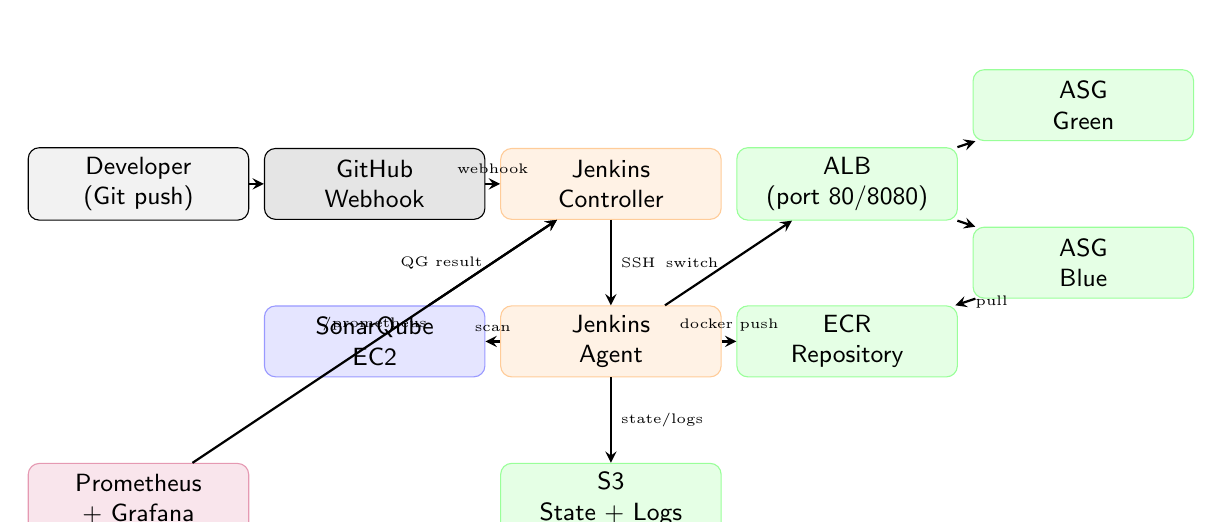
\begin{tikzpicture}[
      box/.style={draw, rounded corners=4pt, minimum width=2.8cm, minimum height=0.9cm,
                  align=center, font=\small\sffamily},
      cloud/.style={box, fill=blue!10, draw=blue!40},
      jenkins/.style={box, fill=orange!10, draw=orange!40},
      aws/.style={box, fill=green!10, draw=green!40},
      monitor/.style={box, fill=purple!10, draw=purple!40},
      arrow/.style={->, >=stealth, thick},
    ]

    % Developer
    \node[box, fill=gray!10] (dev) at (0,0) {Developer\\(Git push)};

    % GitHub
    \node[box, fill=gray!20] (gh) at (3,0) {GitHub\\Webhook};

    % Jenkins Controller
    \node[jenkins] (jc) at (6,0) {Jenkins\\Controller};

    % Jenkins Agent
    \node[jenkins] (ja) at (6,-2) {Jenkins\\Agent};

    % SonarQube
    \node[cloud] (sq) at (3,-2) {SonarQube\\EC2};

    % ECR
    \node[aws] (ecr) at (9,-2) {ECR\\Repository};

    % ALB
    \node[aws] (alb) at (9,0) {ALB\\(port 80/8080)};

    % Blue ASG
    \node[aws] (blue) at (12,-1) {ASG\\Blue};

    % Green ASG
    \node[aws] (green) at (12,1) {ASG\\Green};

    % S3
    \node[aws] (s3) at (6,-4) {S3\\State + Logs};

    % Prometheus + Grafana
    \node[monitor] (obs) at (0,-4) {Prometheus\\+ Grafana};

    % Arrows
    \draw[arrow] (dev) -- (gh);
    \draw[arrow] (gh) -- (jc) node[midway, above, font=\tiny]{webhook};
    \draw[arrow] (jc) -- (ja) node[midway, right, font=\tiny]{SSH};
    \draw[arrow] (ja) -- (sq) node[midway, above, font=\tiny]{scan};
    \draw[arrow] (sq) -- (jc) node[midway, left, font=\tiny]{QG result};
    \draw[arrow] (ja) -- (ecr) node[midway, above, font=\tiny]{docker push};
    \draw[arrow] (ja) -- (alb) node[midway, left, font=\tiny]{switch};
    \draw[arrow] (alb) -- (blue);
    \draw[arrow] (alb) -- (green);
    \draw[arrow] (blue) -- (ecr) node[midway, right, font=\tiny]{pull};
    \draw[arrow] (ja) -- (s3) node[midway, right, font=\tiny]{state/logs};
    \draw[arrow] (obs) -- (jc) node[midway, above, font=\tiny]{/prometheus};

  \end{tikzpicture}
  \caption{End-to-end CI/CD architecture: Jenkins controller delegates to agent, which runs SonarQube scan, builds and pushes Docker image to ECR, and switches the ALB to the new blue/green target. Prometheus and Grafana monitor the controller and agent.}
  \label{fig:arch}
\end{figure}

\newpage
% =============================================================================
\section*{Observability (Bonus)}
% =============================================================================
\addcontentsline{toc}{section}{Observability (Bonus)}

\subsection*{Overview}
Prometheus and Grafana are deployed via Docker Compose
(\texttt{assignment-4/observability/docker-compose.yml}) on the Jenkins
controller or a dedicated monitoring host.

\subsection*{Prometheus Configuration}

\begin{lstlisting}[language=bash, caption={assignment-4/observability/prometheus.yml}]
global:
  scrape_interval: 15s

scrape_configs:
  - job_name: jenkins
    metrics_path: /prometheus
    static_configs:
      - targets: ['<controller-ip>:8080']

  - job_name: node_controller
    static_configs:
      - targets: ['<controller-ip>:9100']

  - job_name: node_agent
    static_configs:
      - targets: ['<agent-private-ip>:9100']
\end{lstlisting}

\subsection*{Grafana Dashboard}

The \textbf{Jenkins: Performance and Health Overview} dashboard (Grafana ID 9964)
is imported and shows:
\begin{itemize}[noitemsep, leftmargin=*]
  \item Build queue depth and executor utilisation.
  \item Build success/failure rate (last 24 h).
  \item CPU and memory usage on controller and agent (via node-exporter).
  \item Active pipeline run count.
\end{itemize}

\newpage
% =============================================================================
\section*{Conclusion}
% =============================================================================
\addcontentsline{toc}{section}{Conclusion}

This assignment demonstrated a production-grade CI/CD pipeline on AWS:

\begin{itemize}[leftmargin=*]
  \item \textbf{Infrastructure as Code}: all resources (EC2, SG, IAM, ECR, ALB, ASG)
        are reproducibly provisioned by Terraform with S3+DynamoDB state locking.
  \item \textbf{Security}: the Jenkins agent runs in a private subnet; container images
        are scanned by Trivy; Terraform configurations are audited by tfsec; no
        plaintext secrets exist in any committed file.
  \item \textbf{Quality}: SonarQube enforces a 70\% coverage gate; 38 tests (unit +
        integration) run in parallel on every push.
  \item \textbf{Reliability}: blue-green deployment with smoke tests ensures zero
        downtime; automatic rollback prevents bad code reaching live traffic.
  \item \textbf{Observability}: Prometheus + Grafana give real-time pipeline health
        visibility alongside CloudWatch.
\end{itemize}

% =============================================================================
\section*{References}
% =============================================================================
\addcontentsline{toc}{section}{References}

\begin{enumerate}[leftmargin=*]
  \item Jenkins Documentation. \url{https://www.jenkins.io/doc/}
  \item HashiCorp Terraform AWS Provider. \url{https://registry.terraform.io/providers/hashicorp/aws/latest}
  \item SonarQube 10 Documentation. \url{https://docs.sonarsource.com/sonarqube/latest/}
  \item Trivy Vulnerability Scanner. \url{https://aquasecurity.github.io/trivy/}
  \item AWS ECR User Guide. \url{https://docs.aws.amazon.com/AmazonECR/latest/userguide/}
  \item AWS ALB Blue/Green Deployments. \url{https://aws.amazon.com/blogs/devops/bluegreen-deployments-with-aws-codedeploy/}
  \item Prometheus Monitoring. \url{https://prometheus.io/docs/introduction/overview/}
  \item Grafana Jenkins Dashboard 9964. \url{https://grafana.com/grafana/dashboards/9964}
\end{enumerate}

\end{document}
